\documentclass{article}
\usepackage{fullpage}
\usepackage{amsmath}
\usepackage{graphicx}
\usepackage{listings}
\usepackage{xcolor}
\usepackage{caption}
\usepackage{subcaption}
 
\definecolor{codegreen}{rgb}{0,0.6,0}
\definecolor{codegray}{rgb}{0.5,0.5,0.5}
\definecolor{codepurple}{rgb}{0.58,0,0.82}
\definecolor{backcolour}{rgb}{0.95,0.95,0.92}
 
\lstdefinestyle{mystyle}{
    backgroundcolor=\color{backcolour},   
    commentstyle=\color{codegreen},
    keywordstyle=\color{magenta},
    numberstyle=\tiny\color{codegray},
    stringstyle=\color{codepurple},
    basicstyle=\ttfamily\footnotesize,
    breakatwhitespace=false,         
    breaklines=true,                 
    captionpos=b,                    
    keepspaces=true,                 
    numbers=left,                    
    numbersep=5pt,                  
    showspaces=false,                
    showstringspaces=false,
    showtabs=false,                  
    tabsize=2,
    xleftmargin=.25in,
}
 
\lstset{style=mystyle}

\renewcommand{\familydefault}{\sfdefault}

\begin{document}
\title{H\"uckel theory using HuLis and Python applied to molecular motors}
\author{Jurn Heinen}
\maketitle
\begin{abstract}
Semi-empirical H\"uckel theory forms an excellent start into molecular quantum chemistry, which is essential in understanding molecular orbital theory. Most quantum chemistry is done using computational resouces. Still most degree programs teach H\"uckel theory using pen and paper. Here, a scientific computational approach is presented that uses an online H\"uckel tool as well as Python programming. By diagonalizing the Hamiltonian matrix, within the H\"uckel framework, the red-shifting of the exciting wavelength of a molecular motor is predicted.
\end{abstract}



\section*{Introduction to H\"uckel theory}
As programming becomes more centralized in educational programs and science in general, it can be argued that students should learn and apply computational methods at an early stage. In this article, I focus on scientific computing applied to molecular quantum chemistry. \cite{Atkins2010} A good starting point is the semi-empirical H\"uckel theory method. \cite{Huckel1931,Huckel1931_2,Huckel1932,Huckel1933}

The wavefunction of a molecular orbital $\phi_i$ is a linear combination of atomic orbitals (AO's) $\chi$
%
\begin{equation}
\phi_i = \sum_{{\mu},i}^N c_{{\mu}i}\chi_{\mu}.
\end{equation}
%

The general form of the secular equations, defined as "the determinant of matrix elements whose solution leads to the set of energy levels of molecular orbitals for a given system."\cite{Minkin2009} can be written as
%
\begin{equation}
\sum_{i=1}^N(h_{ki} - {E}S_{ki})c_i = 0
\end{equation}
%
with $h_{ki}$ is the Hamiltonian, $E$ the energy level of orbital $i$, $S_{ki}$ the overlap matrix between atomic orbitals $k$ and $i$ and $c_i$ the orbital coefficients of the corresponding molecular orbital.
%or in matrix form
%
%\begin{equation}
%(\boldsymbol{h} - {\boldsymbol{\epsilon}}\boldsymbol{S})%\boldsymbol{c_i} = 0
%\end{equation}
%
In H\"uckel molecular orbital (HMO) theory, only $\pi$-electrons are considered and the secular equations are reduced in complexity as the result of the following approximations
%
\begin{enumerate}
\item overlap integrals are set to zero ($S_{ki} = 0$)
\item diagonal elements of the hamiltonian ($h_{ii}$) are set to $\alpha$
\item off-diagonal elements of the hamiltonian corresponding to neighbouring atoms are set to $\beta$
\end{enumerate}
%
The secular equations, in matrix form, are now
%
\begin{equation}
\begin{split}
\boldsymbol{c^{-1}hc} &= \boldsymbol{E} \\
\end{split}
\label{eq:diagonalization}
\end{equation}.
%
This is a typical matrix diagonalization problem.

Matrix diagonalization is a central topic in various computational fields. The process of diagonalizing is equivalent to finding the matrix's eigenvalues and eigenvectors. In other words: by diagonlizing the Hamiltonian, the eigenvalues, which are the energy levels of the molecular orbitals, are obtained. The eigenvectors that diagonalize the Hamiltonian matrix form the coefficients of the molecular orbitals.

\section*{Textbook example: 1,3-butadiene}
Consider a molecular orbital $\phi_i$ of 1,3-butadiene

\begin{equation}
\phi_i = c_{i1}\chi_1 + c_{i2}\chi_2 + c_{i3}\chi_3 + c_{i4}\chi_4.
\end{equation} 

The associated Hamiltonian, within the H\"uckel approximation, is given by
%
\begin{equation}
h =
\begin{pmatrix}
\alpha & \beta & 0 & 0 \\
\beta & \alpha & \beta & 0  \\
0 & \beta & \alpha & \beta  \\
0 & 0 & \beta & \alpha \\
\end{pmatrix}
\end{equation}
%
where the Coulomb ($\alpha$) and resonance ($\beta$) matrices can be split accordingly
%
\begin{equation}
\alpha * \boldsymbol{1} + \beta
\begin{pmatrix}
0 & 1 & 0 & 0 \\
1 & 0 & 1 & 0 \\
0 & 1 & 0 & 1 \\
0 & 0 & 1 & 0 \\
\end{pmatrix}
\end{equation}
%
The Coulomb matrix is already diagonal. Using Python it is straightforward to diagonalize the resonance matrix
%
\begin{lstlisting}[language=Python,label={lst:python_butadiene}]
import numpy as np
from numpy import linalg as LA
\boldsymbol{h} = np.array([
[0, 1, 0, 0],
[1, 0, 1, 0],
[0, 1, 0, 1],
[0, 0, 1, 0]])
E, c = LA.eig(H)
print("Eigenvalues E: \n", E)
print("Eigenvector c: \n", c)
\end{lstlisting}
%
which would give the following result
%
\begin{lstlisting}[language=Python]
Eigenvalues E: 
 [-1.61803399 -0.61803399  1.61803399  0.61803399]
Eigenvector c: 
 [[ 0.37174803  0.60150096 -0.37174803 -0.60150096]
 [-0.60150096 -0.37174803 -0.60150096 -0.37174803]
 [ 0.60150096 -0.37174803 -0.60150096  0.37174803]
 [-0.37174803  0.60150096 -0.37174803  0.60150096]]
\end{lstlisting}
%
Each of the four eigenvalues $E_i$ corresponds to a set of eigenvectors $c_i$. Note, that textbooks or other software might give a different order of the values or alternating positive / negative signs. Also, the eigenvectors are commonly normalized. The calculated eigenvalues correspond to the $\beta$-values. Hence the total orbital energies are
%
\begin{equation}
E = 
\begin{pmatrix}
\alpha + 1.62\beta & 0 & 0 & 0 \\
0 & \alpha + 0.62\beta & 0 & 0  \\
0 & 0 & \alpha - 0.62\beta & 0 \\
0 & 0 & 0 & \alpha - 1.62\beta  \\

\end{pmatrix}
\end{equation}.
%
These numbers are not always immediately intuitive. For this reason, chemists visualize the eigenvectors (the coefficients of the molecular orbitals) and thereby generate molecular orbital pictures. This is shown in Figure \ref{fig:mos_butadiene}. The higher the coefficient, the larger the atomic orbital is drawn. As electrons are distributed according to the Aufbau-principle, and 1,3-butadiene has 4 $\pi$-electrons, the first 2 molecular orbitals are occupied. Remember that the resonance integrals are negative.

\begin{figure}[h]
\centering
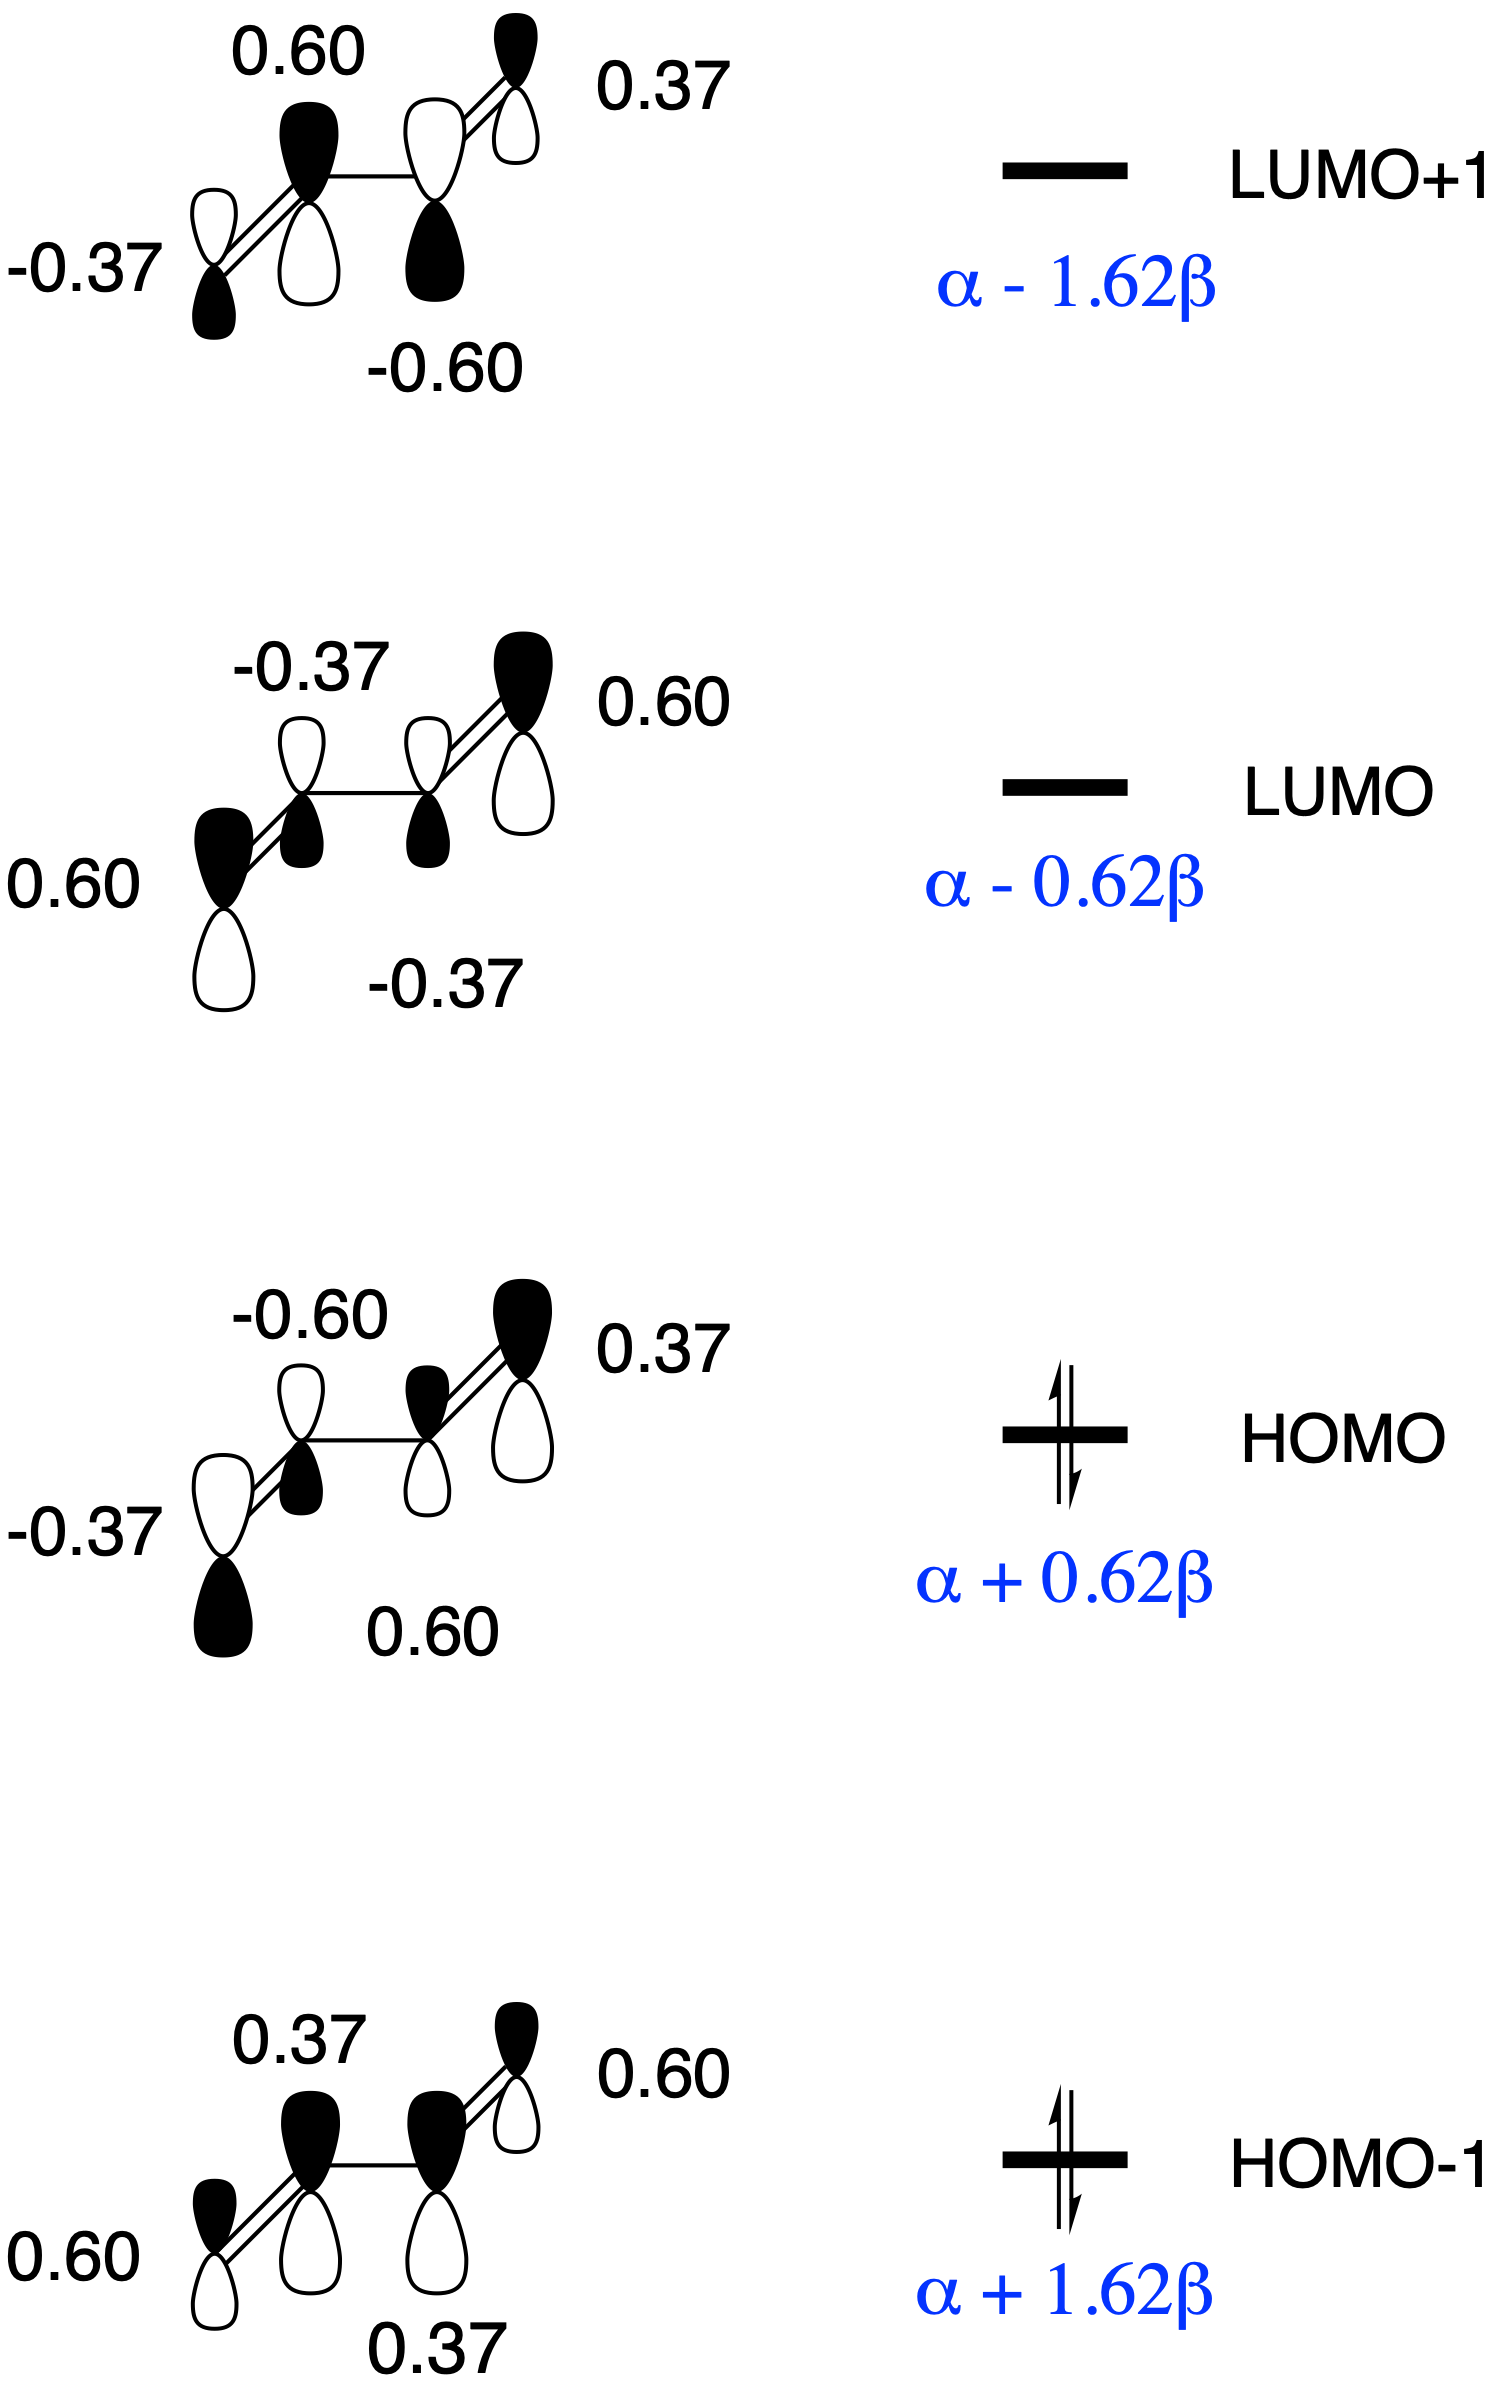
\includegraphics[scale=0.5]{./images/mos_1-3-butadiene.png}
\caption{Molecular orbitals of 1,3-butadiene calculated with HMO theory. Relative size of MO coefficients are drawn scaled.}
\label{fig:mos_butadiene}
\end{figure}



\clearpage
\section*{Symmetry enhanced diagonalization of Hamiltonian}

Molecules belong to a certain point group depending on the symmetry of the nuclei. The symmetry has implications to the electronic structure and speeds up computations. Consider the allyl radical (C$_1$-C$_2$-C$_3$) as shown in figure below

\begin{figure}[h]
\centering
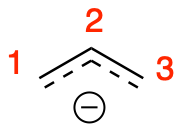
\includegraphics[scale=1.0]{./images/allyl_labels.png}
\caption{Allyl radial with atom labels in red.}
\label{fig:allyl}
\end{figure} 

Without symmetry the Hamiltonian is written as
%
\begin{equation}
\boldsymbol{h} =
\begin{pmatrix}
\alpha & \beta & 0 \\
\beta & \alpha & \beta \\
0 & \beta & \alpha
\end{pmatrix}.
\end{equation}
%
Diagonalizing the resonance matrix, using the same code as in Listing \ref{lst:python_butadiene}, gives
%
\begin{lstlisting}[language=Python]
(array([-1.41421356e+00,  9.77950360e-17,  1.41421356e+00]),
 array([[ 5.00000000e-01,  7.07106781e-01,  5.00000000e-01],
        [-7.07106781e-01,  9.06753788e-17,  7.07106781e-01],
        [ 5.00000000e-01, -7.07106781e-01,  5.00000000e-01]])).
\end{lstlisting}
%
This procedure involves diagonalizing a $3 \times 3$ matrix. If the reflection plane through atom C$_2$ is considered, symmetric and anti-symmetric linear combinations of the atomic orbitals can be constructed. To state this differently, a different basis set is used to span the vector space. In the non-symmetry basis set, the basis functions are denoted $\chi_i$, in the symmetric case this is $\psi_i$.

Within the Cs point group, these are the A' and A'' irreducible representations (irreps), respectively. The A'' Hamiltonian is simply $h^{A''} = \alpha$ and the A'' Hamiltonian is
%
\begin{equation}
h^{A'} = 
\begin{pmatrix}
h_{11}^{A'} & h_{12}^{A'} \\
h_{21}^{A'} & h_{22}^{A'} \\
\end{pmatrix}
=
\begin{pmatrix}
\alpha & \sqrt{2}\beta \\
\sqrt{2}\beta & \alpha \\
\end{pmatrix}.
\end{equation}
%

The diagonalization problem is now reduced considerably.
\clearpage

\section*{Application of H\"uckel theory to predict red-shifting of excition wavelength upon aromatic substitution of a molecular motor}
In 2016, the Chemistry Nobel Prize was awarded to Fraser Stoddart, Jean-Pierre Sauvage and Ben Feringa "for the design and synthesis of molecular machines".\cite{nobelprizechemistry2016} A special type of these molecular machines is the molecular motor. A molecular motors has light-addressable switches and can isomerize under the influence of UV-light.\cite{Feringa2012} The unidirectional rotation of a motor was first reported in 1999 using UV-radiation and thermal relaxation.\cite{Koumura1999} This lead to the radical idea that these molecular motors can be used potentially as nanorobots used in drug delivery. An example is shown in Figure \ref{fig:mm1} of how molecular motor \textbf{1} isomerizes at $\lambda$ = 395 nm.

\begin{figure}[h]
\centering
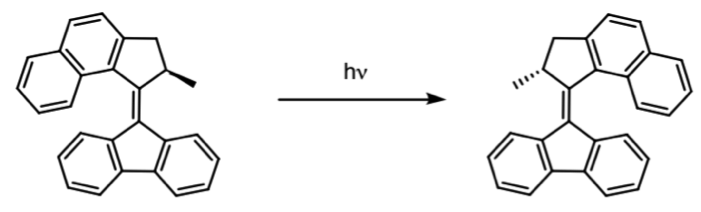
\includegraphics[scale=0.75]{./images/scheme1.png}
\caption{Molecular motor \textbf{1} isomerizes using a wavelength of $\lambda$ = 395 nm.}
\label{fig:mm1}
\end{figure} 

However, UV-light can damage biological matter. Therefore, it is crucial that the excitation wavelength needed for isomerization is reduced to lower wavelengths. A recent experimental study by Feringa et al. showed that extending the aromatic core by substituting the benzene-core by a naphthalene-core, termed motor \textbf{2} as shown in Figure \ref{fig:mm2}, can red-shift the excitation wavelength of the molecular motor.\cite{VanLeeuwen2017} 

\begin{figure}[h]
\centering
\begin{subfigure}[b]{0.5\textwidth}
\centering
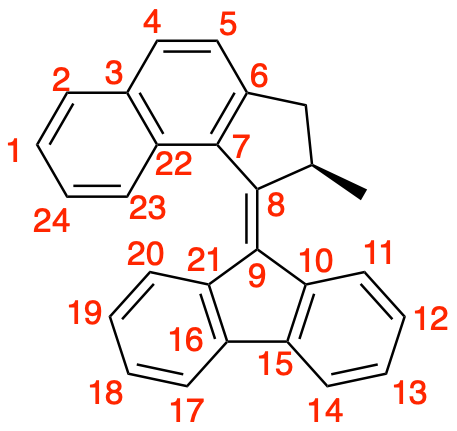
\includegraphics[scale=1.0]{./images/mm1_labels.png}
\caption{Motor \textbf{1}}
\end{subfigure}~
\begin{subfigure}[b]{0.5\textwidth}
\centering
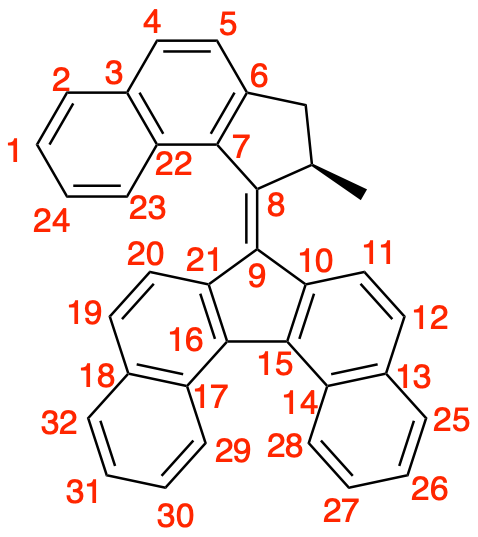
\includegraphics[scale=1.0]{./images/mm2_labels.png}
\caption{Motor \textbf{2}}
\end{subfigure}
\caption{Substitution of the aromatic core of molecular motor \textbf{1} by a naphthalene causes a red-shift of the excitation wavelength to 491 nm.}
\label{fig:mm2}
\end{figure} 

Using H\"uckel theory calculations, this red-shifting can be predicted by comparing the HOMO-LUMO gaps of both motors. In this example, the tool HuLis is used.\cite{Carissan2008, hulis} The HOMO-LUMO gap of motor \textbf{1} is E$_\text{LUMO}$ - E$_\text{HOMO}$ = ($\alpha$ - 0.28$\beta$) - ($\alpha$ + 0.43$\beta$) = -0.71$\beta$. It is expected that the same gap should be calculated for motor \textbf{2}. Feringa et al. found that the HOMO-1 to LUMO excitation has a significant larger oscillator strength (0.6241) compared to the HOMO to LUMO excitation (0.0105) for molecular motor \textbf{2}. A higher oscillation strengths implies a large transition probability for excitation. Therefore, the excitation energy for motor \textbf{2} is calculated from the HOMO-1 LUMO gap and results in ($\alpha$ - 0.21$\beta$) - ($\alpha$ + 0.47$\beta$) = -0.68$\beta$. Since $\beta {<} 0$, the red-shift is indeed predicted. Moreover, visualization of the HOMO, HOMO-1 and LUMO of motors \textbf{1} and \textbf{2}, shown in Figure \ref{fig:hulis_orbitals}, agree surprisingly well with TD-DFT (B3LYP 6-31(d,g)) calculations of Fergina et al.

\begin{figure}[h]
\centering
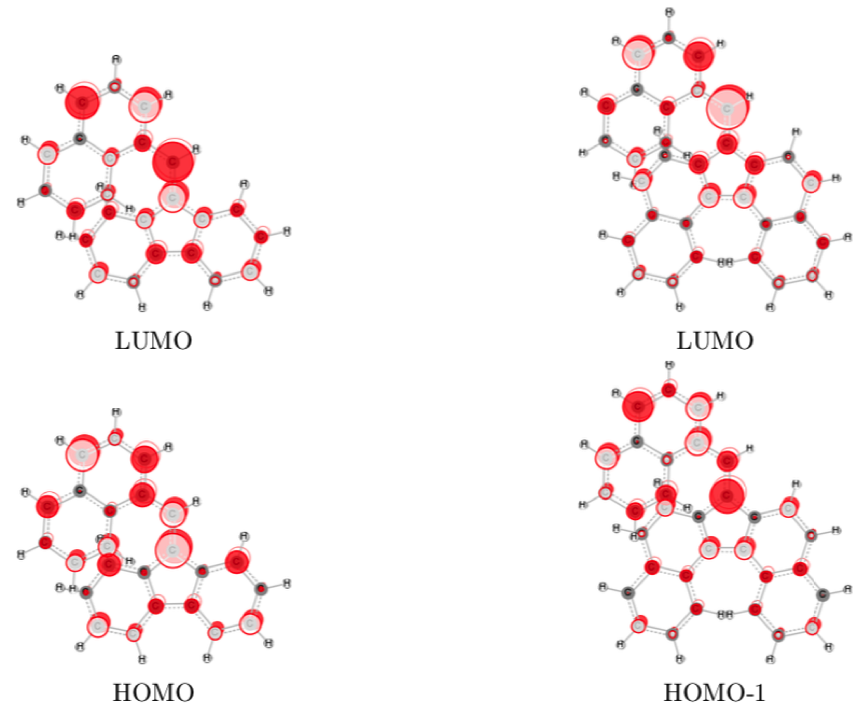
\includegraphics[scale=0.75]{./images/hulis_mm.png}
\caption{Frontier molecular orbitals of motor \textbf{1} (left) and motor \textbf{2} (right) generated with HuLiS.}
\label{fig:hulis_orbitals}
\end{figure} 

HuLis is convenient tool for H\"uckel calculation and visualization. 

In listing \ref{lst:hamiltonian_mm1} and \ref{lst:hamiltonian_mm2} are the $\beta$-matrix for motor \textbf{1} and \textbf{2} shown. The elements of the matrix agree with the atom indices shown in Figure \ref{fig:mm2}. Note that the labels of the atoms (and hence the hamiltonian matrix) are completely arbitrary. Also note that the aliphatic part of the five-ring is not numbered as single bonds are not considered in H\"uckel theory (except in extended H\"uckel theory). Motor \textbf{1} and \textbf{2} contain 24 and 32 $\pi$-electrons, respectively.

\begin{lstlisting}[language=Python,caption={Matrix of the resonance integrals of the Hamiltonian of motor 1},label={lst:hamiltonian_mm1}]
H = np.array([
[0,1,0,0,0,0,0,0,0,0,0,0,0,0,0,0,0,0,0,0,0,0,0,1],   
[1,0,1,0,0,0,0,0,0,0,0,0,0,0,0,0,0,0,0,0,0,0,0,0],
[0,1,0,1,0,0,0,0,0,0,0,0,0,0,0,0,0,0,0,0,0,1,0,0], 
[0,0,1,0,1,0,0,0,0,0,0,0,0,0,0,0,0,0,0,0,0,0,0,0], 
[0,0,0,1,0,1,0,0,0,0,0,0,0,0,0,0,0,0,0,0,0,0,0,0], 
[0,0,0,0,1,0,1,0,0,0,0,0,0,0,0,0,0,0,0,0,0,0,0,0], 
[0,0,0,0,0,1,0,1,0,0,0,0,0,0,0,0,0,0,0,0,0,1,0,0], 
[0,0,0,0,0,0,1,0,1,0,0,0,0,0,0,0,0,0,0,0,0,0,0,0], 
[0,0,0,0,0,0,0,1,0,1,0,0,0,0,0,0,0,0,0,0,1,0,0,0], 
[0,0,0,0,0,0,0,0,1,0,1,0,0,0,1,0,0,0,0,0,0,0,0,0], 
[0,0,0,0,0,0,0,0,0,1,0,1,0,0,0,0,0,0,0,0,0,0,0,0], 
[0,0,0,0,0,0,0,0,0,0,1,0,1,0,0,0,0,0,0,0,0,0,0,0], 
[0,0,0,0,0,0,0,0,0,0,0,1,0,1,0,0,0,0,0,0,0,0,0,0], 
[0,0,0,0,0,0,0,0,0,0,0,0,1,0,1,0,0,0,0,0,0,0,0,0], 
[0,0,0,0,0,0,0,0,0,1,0,0,0,1,0,1,0,0,0,0,0,0,0,0], 
[0,0,0,0,0,0,0,0,0,0,0,0,0,0,1,0,1,0,0,0,1,0,0,0], 
[0,0,0,0,0,0,0,0,0,0,0,0,0,0,0,1,0,1,0,0,0,0,0,0], 
[0,0,0,0,0,0,0,0,0,0,0,0,0,0,0,0,1,0,1,0,0,0,0,0], 
[0,0,0,0,0,0,0,0,0,0,0,0,0,0,0,0,0,1,0,1,0,0,0,0], 
[0,0,0,0,0,0,0,0,0,0,0,0,0,0,0,0,0,0,1,0,1,0,0,0], 
[0,0,0,0,0,0,0,0,1,0,0,0,0,0,0,1,0,0,0,1,0,0,0,0], 
[0,0,1,0,0,0,1,0,0,0,0,0,0,0,0,0,0,0,0,0,0,0,1,0], 
[0,0,0,0,0,0,0,0,0,0,0,0,0,0,0,0,0,0,0,0,0,1,0,1],
[1,0,0,0,0,0,0,0,0,0,0,0,0,0,0,0,0,0,0,0,0,0,1,0], 
])
\end{lstlisting}

\begin{lstlisting}[language=Python,caption={Matrix of the resonance integrals of the Hamiltonian of motor 2},label={lst:hamiltonian_mm2}]
H = np.array([
[0,1,0,0,0,0,0,0,0,0,0,0,0,0,0,0,0,0,0,0,0,0,0,1,0,0,0,0,0,0,0,0], 
[1,0,1,0,0,0,0,0,0,0,0,0,0,0,0,0,0,0,0,0,0,0,0,0,0,0,0,0,0,0,0,0], 
[0,1,0,1,0,0,0,0,0,0,0,0,0,0,0,0,0,0,0,0,0,1,0,0,0,0,0,0,0,0,0,0], 
[0,0,1,0,1,0,0,0,0,0,0,0,0,0,0,0,0,0,0,0,0,0,0,0,0,0,0,0,0,0,0,0], 
[0,0,0,1,0,1,0,0,0,0,0,0,0,0,0,0,0,0,0,0,0,0,0,0,0,0,0,0,0,0,0,0], 
[0,0,0,0,1,0,1,0,0,0,0,0,0,0,0,0,0,0,0,0,0,0,0,0,0,0,0,0,0,0,0,0], 
[0,0,0,0,0,1,0,1,0,0,0,0,0,0,0,0,0,0,0,0,0,1,0,0,0,0,0,0,0,0,0,0], 
[0,0,0,0,0,0,1,0,1,0,0,0,0,0,0,0,0,0,0,0,0,0,0,0,0,0,0,0,0,0,0,0], 
[0,0,0,0,0,0,0,1,0,1,0,0,0,0,0,0,0,0,0,0,1,0,0,0,0,0,0,0,0,0,0,0], 
[0,0,0,0,0,0,0,0,1,0,1,0,0,0,1,0,0,0,0,0,0,0,0,0,0,0,0,0,0,0,0,0], 
[0,0,0,0,0,0,0,0,0,1,0,1,0,0,0,0,0,0,0,0,0,0,0,0,0,0,0,0,0,0,0,0], 
[0,0,0,0,0,0,0,0,0,0,1,0,1,0,0,0,0,0,0,0,0,0,0,0,0,0,0,0,0,0,0,0], 
[0,0,0,0,0,0,0,0,0,0,0,1,0,1,0,0,0,0,0,0,0,0,0,0,1,0,0,0,0,0,0,0], 
[0,0,0,0,0,0,0,0,0,0,0,0,1,0,1,0,0,0,0,0,0,0,0,0,0,0,0,1,0,0,0,0], 
[0,0,0,0,0,0,0,0,0,1,0,0,0,1,0,1,0,0,0,0,0,0,0,0,0,0,0,0,0,0,0,0], 
[0,0,0,0,0,0,0,0,0,0,0,0,0,0,1,0,1,0,0,0,1,0,0,0,0,0,0,0,0,0,0,0], 
[0,0,0,0,0,0,0,0,0,0,0,0,0,0,0,1,0,1,0,0,0,0,0,0,0,0,0,0,1,0,0,0], 
[0,0,0,0,0,0,0,0,0,0,0,0,0,0,0,0,1,0,1,0,0,0,0,0,0,0,0,0,0,0,0,1], 
[0,0,0,0,0,0,0,0,0,0,0,0,0,0,0,0,0,1,0,1,0,0,0,0,0,0,0,0,0,0,0,0], 
[0,0,0,0,0,0,0,0,0,0,0,0,0,0,0,0,0,0,1,0,1,0,0,0,0,0,0,0,0,0,0,0], 
[0,0,0,0,0,0,0,0,1,0,0,0,0,0,0,1,0,0,0,1,0,0,0,0,0,0,0,0,0,0,0,0], 
[0,0,1,0,0,0,1,0,0,0,0,0,0,0,0,0,0,0,0,0,0,0,1,0,0,0,0,0,0,0,0,0], 
[0,0,0,0,0,0,0,0,0,0,0,0,0,0,0,0,0,0,0,0,0,1,0,1,0,0,0,0,0,0,0,0], 
[1,0,0,0,0,0,0,0,0,0,0,0,0,0,0,0,0,0,0,0,0,0,1,0,0,0,0,0,0,0,0,0], 
[0,0,0,0,0,0,0,0,0,0,0,0,1,0,0,0,0,0,0,0,0,0,0,0,0,1,0,0,0,0,0,0], 
[0,0,0,0,0,0,0,0,0,0,0,0,0,0,0,0,0,0,0,0,0,0,0,0,1,0,1,0,0,0,0,0], 
[0,0,0,0,0,0,0,0,0,0,0,0,0,0,0,0,0,0,0,0,0,0,0,0,0,1,0,1,0,0,0,0], 
[0,0,0,0,0,0,0,0,0,0,0,0,0,1,0,0,0,0,0,0,0,0,0,0,0,0,1,0,0,0,0,0], 
[0,0,0,0,0,0,0,0,0,0,0,0,0,0,0,0,1,0,0,0,0,0,0,0,0,0,0,0,0,1,0,0], 
[0,0,0,0,0,0,0,0,0,0,0,0,0,0,0,0,0,0,0,0,0,0,0,0,0,0,0,0,1,0,1,0], 
[0,0,0,0,0,0,0,0,0,0,0,0,0,0,0,0,0,0,0,0,0,0,0,0,0,0,0,0,0,1,0,1], 
[0,0,0,0,0,0,0,0,0,0,0,0,0,0,0,0,0,1,0,0,0,0,0,0,0,0,0,0,0,0,1,0], 
])
\end{lstlisting}

The Python (Numpy) library $linalg.eiv$ originates from the \_geev routine in LAPACK. Here, a matrix $A$ is reduced to upper Hessenberg form $F$. The matrix $F$ is factorized using Schur decomposition into matrix $T$ for which the eigenvalues and eigenvectors are determined. The LAPACK library is used in most scientific software that performs computations. 

Clearly, these calculations are computationally cheap. This has multiple reasons. First of all, overlap integrals are not calculated, no real basis set, no real computation of hamiltonian elements.

\clearpage

\bibliographystyle{unsrt}               
\bibliography{references.bib}    

\end{document}
